\section{Methodology}
\label{sec:method}

The three tasks share one signal model, one noise model and one scoring harness,
and every method is scored on the same realisation. The protocol differs from
the first version in two places: the truth is drawn from two families, one inside
and one outside the parametric basis, and detection is additionally scored
against real catalogue labels. Table~\ref{tab:methods} collects the methods and
their costs; the text gives only what the table cannot. Fig.~\ref{fig:pipeline}
shows how the stages connect: the same frozen realisation feeds every candidate,
and every candidate is carried through to the velocity product.

\subsection{Signal and noise model}
\label{sec:method:model}

A coordinate component is modelled as
\begin{equation}
y(t) = x(t) + \varepsilon(t), \qquad t\in[t_0,t_0+T],
\label{eq:obs}
\end{equation}
on a daily grid ($\Delta t=1/365.25$~yr), with
\begin{equation}
\label{eq:signal}
\begin{aligned}
x(t) =\;& v\,(t-t_0)
+ S_1\bigl[1+a_m\sin(2\pi f_m(t-t_0)+\phi_m)\bigr]
\sin(2\pi(t-t_0)+\phi_1) \\
&+ S_2\sin(4\pi(t-t_0)+\phi_2)
+ \sum_k b_k H(t-e_k) \\
&+ \sum_j c_j H(t-e_j)e^{-(t-e_j)/\tau_j},
\end{aligned}
\end{equation}
where $H$ is the Heaviside step and $v$ is the secular velocity. The stochastic
term is power-law noise with spectral density
\begin{equation}
S(f)=\sigma_{\rm WN}^2+\sigma_{\rm FN}^2\Bigl(\frac{f_0}{f}\Bigr)
+\sigma_{\rm RW}^2\Bigl(\frac{f_0}{f}\Bigr)^2,
\label{eq:psd}
\end{equation}
generated by inverse Fourier synthesis on a fixed frequency grid. The primary
experiments set $\sigma_{\rm WN}=1.5$~mm and $\sigma_{\rm FN}=3.0$~mm with
$\sigma_{\rm RW}=0$; the random-walk arm adds $\sigma_{\rm RW}=1.0$~mm.

\subsection{Ground-truth protocol}
\label{sec:method:inject}

The deterministic signal is never known on a real station, so it is created by
injection. Two families are used for every denoising and gap-filling score.

\emph{In-family.} The trend and harmonic amplitudes of Eq.~\eqref{eq:signal} are
taken from a robust fit of the real series, with a mild amplitude modulation
($a_m=0.35$). This is the family the trajectory model assumes, up to the
modulation.

\emph{Out-of-family.} The same station fit is used for the trend and mean
amplitudes, but the annual term receives strong multi-year modulation
($a_m\in[0.6,1.0]$), one or two long-lived exponential transients with decay
times of 0.3--1.5 years are added, and a logarithmic post-seismic relaxation is
included for some stations. These structures cannot be represented by constant
harmonics. The truth is still the deterministic part, so recovery error remains
exact.

Both families are also realised on a fully synthetic grid that sweeps the
parameters beyond what the station set contains. The learned models are always
scored by the network trained on the matching family, so an out-of-family score
is not an artefact of testing an in-family network on unfamiliar structure.

\paragraph{Tasks.}
\emph{T1 denoising} leaves $y$ intact and asks for $\hat{x}$. \emph{T2 gap
filling} removes contiguous blocks of $L\in\{5,10,30,60,120,365\}$ days and asks
for the missing values. \emph{T3 offset detection} adds offsets of amplitude
$A\in\{2,4,8,16,25\}$~mm at epochs at least two years apart and asks for the
epoch list; the real-label arm instead uses the catalogue epochs of
Sec.~\ref{sec:data}. For the real-label arm the match tolerance is 180 days to
allow for catalogue dates that refer to the earthquake rather than to the
observable break, and the minimum separation is 60 days; synthetic detection uses
a 30-day tolerance and 45-day separation, because its truth is exact.

\subsection{Methods}
\label{sec:method:methods}

Table~\ref{tab:methods} lists the classical and learned arms. All classical
methods are deterministic given $(t,y)$ and are fitted on the data they are
applied to. The trajectory model is an iteratively reweighted robust fit of trend
plus constant annual and semiannual harmonics. The Kalman/RTS smoother uses the
same basis with a small process noise. SSA embeds the series in a Hankel matrix
and reconstructs from its leading components; gap filling uses the iterative
variant. Wavelet shrinkage uses a db4 transform and soft thresholding at the
VisuShrink level. Interpolators are piecewise linear and shape-preserving cubic
(PCHIP); a natural cubic spline is not used because it overshoots multi-week gaps.
The classical detector is a greedy two-sample scan of the robust residual: the
epoch with the largest standardised step is accepted, its neighbourhood is
suppressed, the design is augmented, and the search repeats until the statistic
falls below threshold. To put both detector families on the same footing, both
are reduced to a decision field (the classical step statistic and the network
output) and read out by the same threshold-plus-minimum-separation rule; this
allows full precision--recall curves rather than a comparison of two hand-tuned
operating points.

\paragraph{Learned arms.}
The primary network is a one-dimensional U-Net with a contracting encoder and
an expanding decoder, skip connections and $2^3$-fold pooling (base width 12, depth 3,
213\,385 parameters; Fig.~\ref{fig:unet}); one network is trained per task. The
second architecture is a temporal convolutional network with residual blocks,
kernel width 5, channel widths 40--80 and dilations 1, 2, 4, 8 and 16, giving
227\,537 parameters. Both are trained under the identical generator, budget
(3000 steps, batch 32, learning rate $2\times10^{-3}$), window length (1024 days)
and seed list, so architecture and seed effects are not confounded with training
protocol. Denoising and gap filling use ten seeds for each architecture;
detection uses twenty U-Net seeds and ten TCN seeds. A small bidirectional GRU
from the first version (four seeds) is reported only as a sensitivity check.

\begin{figure}[t]
\centering
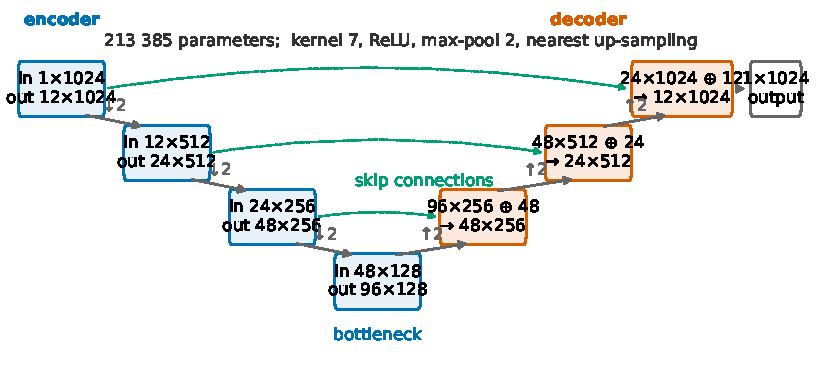
\includegraphics[width=\linewidth]{figures/fig03_unet.pdf}
\caption{The one-dimensional U-Net scored in the primary learned arm. Three
encoder stages halve the resolution and double the width (12 to 96 channels),
the decoder restores it with nearest-neighbour up-sampling, and skip connections
carry the fine-scale detail across the bottleneck. The network has 213\,385
parameters and is trained separately for each task.}
\label{fig:unet}
\end{figure}

Training draws a fresh window at every step. Inputs and targets are standardised
by robust per-window statistics; the detector additionally high-passes the input
and divides by a robust noise scale, so offset amplitude enters as a
signal-to-noise ratio. Long series are processed with 50\% overlapping windows
and averaged. At scoring time each window is standardised by its own statistics
and the network output is transformed back with the same statistics, so the
normalisation at inference matches the one used in training. The whole-series
normalisation of the first version is kept only as an ablation. The gap filler receives the observation mask as a second input
channel. The training distribution covers gaps of 5--120 days, offset amplitudes
in $[-12,12]$~mm and $\sigma_{\rm WN}\in[0.5,3]$~mm,
$\sigma_{\rm FN}\in[0,5]$~mm; the 365-day gap and the 16--25~mm amplitudes are at
or beyond that support and are read as extrapolation.

\begin{table*}[t]
\centering
\caption{Methods compared. ``Field'' denotes the decision field used for
detection; cost is per series unless stated. Parameter counts are for the
learned models; training wall-clock is for one seed on one V100.}
\label{tab:methods}
\footnotesize
\setlength{\tabcolsep}{2.5pt}
\begin{tabularx}{\textwidth}{@{}p{2.05cm}p{1.45cm}Xp{2.2cm}p{1.4cm}p{2.0cm}@{}}
\toprule
Method & Class & Key assumption & Input $\to$ output & Cost & Reference \\
\midrule
Trajectory MLE & parametric & trend + constant harmonics, power-law noise & $y\to\hat{x}$; velocity, $\sigma_v$ & closed form, $<$1~s & \citet{williams2003coloured} \\
Kalman/RTS & parametric & harmonic state, small process noise & $y\to\hat{x}$ & $<$1~s & \\
SSA & model-free & low-rank Hankel structure & $y\to\hat{x}$; gap fill & $<$1~s & \citet{wdowinski1997spatial,ji2024ssa} \\
Wavelet & model-free & sparsity in db4 domain & $y\to\hat{x}$ & $<$1~s & \citet{ji2020wavelet} \\
Moving median & model-free & local smoothness & $y\to\hat{x}$ & $<$1~s & \\
Linear/PCHIP & interp. & local continuity & $y$, mask $\to\hat{x}$ & $<$1~s & \\
Step scan & hyp.\ test & piecewise-constant level & $y\to$ epochs & $<$1~s & \citet{gazeaux2013detecting} \\
U-Net & learned & convolutional encoder--decoder & $y$(+mask) $\to\hat{x}$ or field & 213\,385; 8~min & \citet{ronneberger2015unet} \\
TCN & learned & dilated temporal convolutions & $y$(+mask) $\to\hat{x}$ or field & 227\,537; 6~min & \citet{bai2018tcn} \\
BiGRU & learned & recurrent encoder--decoder & $y\to\hat{x}$ & 182\,785; 5.1~h & \\
\bottomrule
\end{tabularx}
\end{table*}

\subsection{Metrics}
\label{sec:method:metrics}

For T1 the error is $\mathrm{RMSE}(\hat{x},x)$ and the reported quantity is the
reduction $1-\mathrm{RMSE}/\mathrm{RMSE}_{\rm none}$ relative to the undenoised
series. For T2 the error is the RMSE at the masked epochs against the withheld
observation $y$, the value the station recorded; where stated we also report the
error against the noise-free signal $x$, which separates recovering the signal
from reproducing correlated noise. For T3, predicted epochs are greedily matched
to true epochs within the task tolerance, and precision, recall, $F_1$ and average
precision follow. Detection delay is the signed difference between the matched
prediction and the true epoch.

\subsection{Downstream propagation}
\label{sec:method:downstream}

For every method we fit the velocity on its output with the same estimator: the
trend coefficient of the robust trajectory fit and its generalised-least-squares
covariance under a power-law spectrum \citep{williams2008cats,bos2008fast},
\begin{equation}
\hat v=(X^\top C^{-1}X)^{-1}X^\top C^{-1}y,\qquad
\hat\sigma_v^2=\bigl[(X^\top C^{-1}X)^{-1}\bigr]_{vv},
\label{eq:downstream}
\end{equation}
with the WN, FN and RW amplitudes obtained by Whittle maximum likelihood on the
periodogram. Two covariance arms are computed. In the primary (raw-noise) arm the
noise amplitudes are estimated once on the untreated series and held fixed for
every method, so the methods differ only in the series they hand to the velocity
fit. In the secondary (naive) arm the noise is re-estimated on each method's
output; this is the protocol of the first version, and it fails for
model-based denoisers because their output retains no residual from which a
noise amplitude can be recovered. Because the injected velocity is known, the
empirical scatter of $\hat v$ across realisations is compared with the median
reported $\hat\sigma_v$. Their ratio is the calibration ratio (one is honest,
below one is optimistic), and we also report the empirical coverage of the
nominal one- and two-sigma intervals. The random-walk arm repeats the whole chain
with $\sigma_{\rm RW}=1.0$~mm\,yr$^{-1/2}$ and a three-component noise model.
